\testCom
{%Номер задачи
	3.118
}
{%Условие
	условие
}
{%Дано
	дано
}
{%Найти
	найти
}
{%Решение
	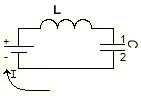
\includegraphics[height=30mm]{3_118.jpg}\\
	$\varphi_2 - \varphi_1 = \frac{q}{c} = \xi - L \der{q}{t}{2}$\\
	$\der{q}{t}{2} + \frac{1}{LC} g = \frac{\xi}{L} \quad \assume g = \tilde g + C' \quad C' = C\xi$\\
	$\der{(\tilde g + C)}{t}{2} + \frac{1}{LC} \tilde g = \frac{\epsilon}{L} - \frac{C'}{LC}$\\
	$\tilde g = C_1 \cos (\omega t + \alpha), \quad \omega = \frac{1}{\sqrt{LC}}$\\
	$\assume \alpha = \frac{3 \pi}{2}, C_1 = C \xi$\\
	$q(t) = C \xi (1 + \sin \omega t) \quad I = \xi \sqrt{\frac{C}{L}} \cos \omega t = \der{q}{t}{}$\\
	$I_{max} = \xi \sqrt{\frac{C}{L}}, U_{max} = \frac{q_{max}}{C} = 2 \xi$\\
}

